\setAuthor{Andreas Valdmann}
\setRound{lõppvoor}
\setYear{2011}
\setNumber{G 8}
\setDifficulty{9}
\setTopic{Geomeetriline optika}

\prob{Optiline süsteem}
Klaasist murdumisnäitajaga $n$ on valmistatud õhuke kaksikkumer lääts, mille mõlema pinna kõverusraadius on $r$ (läätse paksus
$d \gg r$). Läätse üks pind kaetakse peegeldava metallikihiga. Leidke kumerläätsest ja nõguspeeglist tekkinud optilise süsteemi fookuskaugus. 

\emph{Vihje}. Fookuskauguse leidmiseks võib vaadelda optilise peatelje lähedasi kiiri, mis levivad
selle suhtes väikese nurga all. Sel juhul saab rakendada väikeste nurkade valemit $\sin \alpha \approx \tan \alpha \approx \alpha$, kus $\alpha$ on radiaanides. 

\hint
Lisaks väikeste nurkade lähendusele lihtsustab ülesande geomeetriat võimalikult sümmeetriliste kiirte käikude uurimist. Näiteks on mugav vaadelda kiiri, mis peegelduvad risti peegli pinnaga.

\solu
\begin{center}
	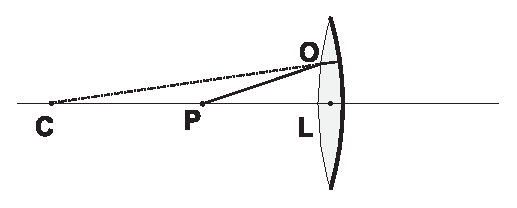
\includegraphics{2011-v3g-08-opt_syst1}
\end{center}

Iga süsteemile langev valguskiir murdub läätse eesmisel pinnal, peegeldub tagumisel pinnal ja murdub uuesti. Lahenduse lihtsustamiseks vaatleme olukorda, kus kiirte käik on sümmeetriline. Sel juhul langeb murdunud kiir peegelpinnale risti, peegeldub otse tagasi ja teine murdumine on esimesega identne. Süsteemi sisenev ja sealt väljuv kiir lõikavad optilist peatelge ühes ja samas punktis $P$. Seal asuva punktobjekti kujutis langeb kokku objekti endaga.

\begin{center}
	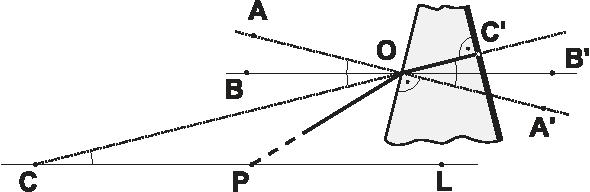
\includegraphics{2011-v3g-08-opt_syst2}
\end{center}

Võtame vaatluse alla teljelähedase kiire $PO$, mille korral võime nurga $\angle LPO$ lugeda väikeseks. Lõik $OC'$ on optilise peateljega veelgi väiksema nurga all ja punktide $O$ ning $C'$ kaugus optilisest peateljest on ligikaudu võrdne. Uurime lähemalt läätse õhukest kihti, mille kõrgus on palju väiksem kõverusraadiusest $r$. Sel juhul võime kõverpinnad asendada nende puutujatega. Pindade ristsirged on joonisel tähistatud punktiirjoonega ning need lõikavad optilist peatelge läätse kõverustsentrites. Optiline kõrvaltelg $BB'$ on paralleelne optilise peateljega ning 
\[
\angle LCO=\angle B'OC'=\angle A'OB'=\angle BOC=\angle AOB\equiv \phi
\]
ja murdumisnurk $\angle A'OC'=2\phi$. Langemisnurgaks on $\angle AOP$. Murdumisseaduse rakendamisel kasutame väikese nurga lähendust 
\[
\frac{\sin(\angle AOP)}{\sin(\angle A'OC')}=n\approx \frac{\angle AOP}{\angle A'OC'},
\]
millest
\[
\angle AOP = n \angle A'OC'=2n\phi.
\]
Järgmisteks arvutusteks on vaja teada nurka
\[
\angle LPO=\angle BOP=\angle AOP - \angle AOB=2n\phi-\phi=(2n-1)\phi.
\]
Kuna lääts on õhuke ja punkt $O$ ei ole kaugel optilisest peateljest, siis $|CO|\approx|CL|$ ja $|PO|\approx|PL|$ ning $|CL|=r-\frac{d}{2}\approx r$, kus $d$ on läätse paksus keskkohas. Jällegi väikese nurga lähendust kasutades saame
\[
|LO|=\angle LCO|CL|=\angle LPO|PL|,
\]
millest
\[
|PL|=\frac{\angle LCO}{\angle LPO}|CL|=\frac{\phi}{(2n-1)\phi} r=\frac{r}{2n-1}.
\]
Viimaseks rakendame läätse valemit
\[
\frac{1}{a}+\frac{1}{k}=\frac{1}{f}
\]
ja seost
\[
|PL|=a=k=\frac{r}{2n-1}
\]
ning saame, et
\[
f=\frac{|PL|}{2}=\frac{r}{2(2n-1)}.
\]
\probend